\chapter{Introduction}
\label{c:intro}

\newcommand{\FourQueens}[2] {
  \begin{tikzpicture}[scale=0.6, every node/.style={black,scale=0.9}]
    \newcommand*{\xMin}{0}%
    \newcommand*{\xMax}{3}%
    \newcommand*{\yMin}{0}%
    \newcommand*{\yMax}{3}%
    \foreach \i / \label in {0/a,1/b,2/c,3/d} {
        \draw [] node at (\i+.5,\yMin-.3) {$\label$};
    }
    \foreach \i / \label in {0/1,1/2,2/3,3/4} {
        \draw [] node at (\xMin-.3,\i+.5) {$\label$};
    }

    \foreach \y in {0,2}{
        \foreach \x in {0,2}{
            \fill[black!8] (\x,\y) rectangle (1+\x,1+\y) rectangle (2+\x,2+\y);}}
    \draw [step=1.0] (0,0) grid (4,4);
    \foreach \x/\y/\m in {#2}
        \draw [] node at (\x,\y) {\m};
    \node[draw,circle,inner sep=1mm] at (-1.4,3.5) {#1};
  \end{tikzpicture}
}

\newcommand{\MCSDomains}[2] {
  \begin{tikzpicture}[scale=0.6, every node/.style={black,scale=0.9}]
    \newcommand*{\xMin}{0}%
    \newcommand*{\xMax}{5}%
    \newcommand*{\yMin}{0}%
    \newcommand*{\yMax}{4}%
    \foreach \i / \label in {0/a,1/b,2/c,3/d,4/e,5/f} {
        \draw [] node at (\i+.5,\yMax+1.4) {$\label$};
    }
    \foreach \i / \label in {4/1,3/2,2/3,1/4,0/5} {
        \draw [] node at (\xMin-.3,\i+.5) {$\label$};
    }

    \draw [step=1.0] (0,0) grid (6,5);
    \foreach \x/\y/\m in {#2}
        \draw [] node at (\x,\y) {\m};
    \node[draw,circle,inner sep=1mm] at (-1.4,3.5) {#1};
  \end{tikzpicture}
}

Graphs, or networks --- collections of items (vertices), some pairs of which
are related --- are a concept that can be used for modelling a huge
range of systems.  We can, for example, view a molecule as a collection
of vertices (the atoms) joined together by bonds
\citep{sussenguth1965graph}; 
an image may be summarised using a vertex for each coloured region
and joining adjacent regions \citep{DBLP:conf/icip/OlatunbosunDE96}.
We may wish to determine whether all or a large
part of a given object --- such as a molecule or image --- is contained
in another given object.  This dissertation presents new algorithms
for such problems.

This dissertation introduces algorithms for three NP-hard problems that
take graphs as inputs.  The first of these is the \emph{maximum common induced subgraph}
family of problems: we seek to find a large subgraph shared by two given graphs.
Depending on the flavour of the problem, these
graphs may be directed or undirected and may or may not have labels.
All of these variants of the can be handled by the \McSplit\ family of algorithms.
These algorithms use a simple, fast and space-efficient data structure to keep
track of the set of vertices in the second graph to which a given vertex
in the first graph may be mapped.

The second problem we consider is \emph{induced subgraph isomorphism}: to determine
whether a given graph (the ``target graph'') contains another given graph (the ``pattern graph'')
as an induced subgraph.  We again use a variant of the \McSplit\ algorithm ---
\McSplit-SI --- to solve the problem; this version of the algorithm has a specialised
version of \McSplit's data structure that allows very fast processing of sparse graphs.

For the final problem considered in this dissertation, we turn from subgraphs
to supergraphs.  We study the problem of finding, for a given family of graphs
an \textit{induced universal graph} --- that is, a graph that contains every
member of the family as an induced subgraph --- with as few vertices as
possible.  This problem generalises the \textit{minimum common supergraph}
problem to an arbitrary number of input graphs.  Although much progress has
been made on asymptotic results on the size of induced universal graphs, little
work has been done on developing algorithms to solve the problem exactly.  This
dissertation presents an algorithm for finding minimal induced universal graphs
using \McSplit-SI as a subroutine, and presents new terms of integer sequences
generated using the program.  Further, we present a hill-climbing method for
finding small (but possibly not optimal) induced universal graphs.

%The final problem covered in this dissertation is the treedepth problem: the
%problem of finding a \textit{treedepth decomposition} of minimum height for a given
%graph.  TODO say more

%This paper introduces a family of algorithms for finding maximum common
%substructures in a broad class of objects that includes both graphs and
%hypergraphs.

\section{Maximum Common Induced Subgraph}

We begin with a the maximum common induced subgraph (MCIS) problem. A
graph $G$ is a pair $(V, E)$, where $V = V(G)$ is the vertex set and $E = E(G)$
is the edge set. Each element of $E$ is a two-element subset of $V$, whose
elements are referred to as its endpoints. For example, suppose we have
\[
V = \{1, 2, 3, 4, 5, 6\},
E = \{\{1,2\}, \{1,3\}, \{2,3\}, \{3,4\}, \{4,5\}, \{4,6\}, \{5,6\}\}
.
\]
This graph may be drawn as shown in \Cref{fig:introA}, with a point for each
vertex and a line for each edge.  The positions of the points in the plane have
no significance.

\begin{figure}[h!]
\centering
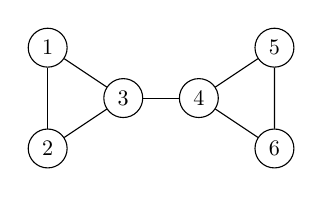
\begin{tikzpicture}[scale=0.8, every node/.style={scale=0.8}]
%\begin{tikzpicture}
  \node [draw,circle] (1) at (0,1.6) {1};
  \node [draw,circle] (2) at (0,0) {2};
  \node [draw,circle] (3) at (1.2,.8) {3};
  \node [draw,circle] (4) at (2.4,.8) {4};
  \node [draw,circle] (5) at (3.6,1.6) {5};
  \node [draw,circle] (6) at (3.6,0) {6};
  \draw (1) -- (2);
  \draw (1) -- (3);
  \draw (2) -- (3);
  \draw (3) -- (4);
  \draw (4) -- (5);
  \draw (4) -- (6);
  \draw (5) -- (6);
\end{tikzpicture}
\caption{A graph}
\label{fig:introA}
\end{figure}

Two graphs are isomorphic if they can be drawn identically. Thus, the graph in
Figure B is isomorphic to the graph in \Cref{fig:introA}, despite having a different
vertex set. Formally, an isomorphism between graphs $G$ and $H$ is a bijection $f$
between the vertex set of $G$ and the vertex set of $H$, such that if we apply $f$ to
the endpoints of each edge of $G$ we obtain the edge set of $H$. If such an $f$
exists, we say that $G$ and $H$ are isomorphic.

\begin{figure}[h!]
\centering
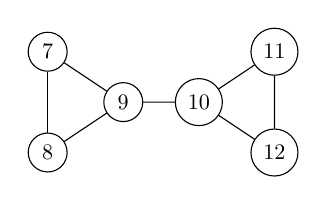
\begin{tikzpicture}[scale=0.8, every node/.style={scale=0.8}]
%\begin{tikzpicture}
  \node [draw,circle] (1) at (0,1.6) {7};
  \node [draw,circle] (2) at (0,0) {8};
  \node [draw,circle] (3) at (1.2,.8) {9};
  \node [draw,circle] (4) at (2.4,.8) {10};
  \node [draw,circle] (5) at (3.6,1.6) {11};
  \node [draw,circle] (6) at (3.6,0) {12};
  \draw (1) -- (2);
  \draw (1) -- (3);
  \draw (2) -- (3);
  \draw (3) -- (4);
  \draw (4) -- (5);
  \draw (4) -- (6);
  \draw (5) -- (6);
\end{tikzpicture}
\caption{Figure B TODO: add caption}
\end{figure}

An induced subgraph of $G = (V, E)$ has a subset $W$ of $V$ as its vertex set, and
$\{\{u, v\} \in E \mid u, v \in W\}$ as its edge set; that is, the subgraph
includes all edges of $G$ both of whose endpoints appear in $W$.  The first graph
in Figure C is thus an induced subgraph of the graph in Figure A, whereas the
second graph is not. We say that the set $W$ induces the subgraph.

\begin{figure}[h!]
\centering
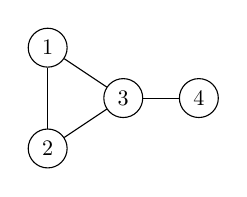
\begin{tikzpicture}[scale=0.8, every node/.style={scale=0.8}]
  \node [draw,circle] (1) at (0,1.6) {1};
  \node [draw,circle] (2) at (0,0) {2};
  \node [draw,circle] (3) at (1.2,.8) {3};
  \node [draw,circle] (4) at (2.4,.8) {4};
  \draw (1) -- (2);
  \draw (1) -- (3);
  \draw (2) -- (3);
  \draw (3) -- (4);
\end{tikzpicture}
\qquad
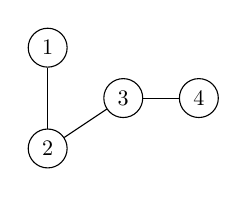
\begin{tikzpicture}[scale=0.8, every node/.style={scale=0.8}]
  \node [draw,circle] (1) at (0,1.6) {1};
  \node [draw,circle] (2) at (0,0) {2};
  \node [draw,circle] (3) at (1.2,.8) {3};
  \node [draw,circle] (4) at (2.4,.8) {4};
  \draw (1) -- (2);
  \draw (2) -- (3);
  \draw (3) -- (4);
\end{tikzpicture}
\caption{Figure C TODO: add caption}
\end{figure}

A \emph{common induced subgraph} of graphs $G$ and $H$ is an induced subgraph of $G$ which
is isomorphic to an induced subgraph of $H$. In figure D, a common induced
subgraph of the two graphs is shown in bold on the first graph, and its
isomorphic subgraph is shown in bold on the second graph.

\begin{figure}[h!]
\centering
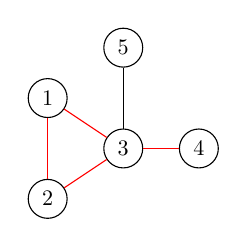
\begin{tikzpicture}[scale=0.8, every node/.style={scale=0.8}]
  \node [draw,circle] (1) at (0,1.6) {1};
  \node [draw,circle] (2) at (0,0) {2};
  \node [draw,circle] (3) at (1.2,.8) {3};
  \node [draw,circle] (4) at (2.4,.8) {4};
  \node [draw,circle] (5) at (1.2,2.4) {5};
  \draw [red] (1) -- (2);
  \draw [red] (1) -- (3);
  \draw [red] (2) -- (3);
  \draw [red] (3) -- (4);
  \draw (3) -- (5);
\end{tikzpicture}
\qquad
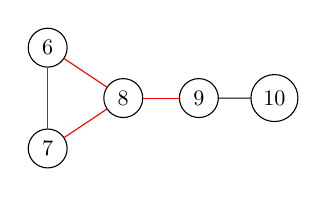
\begin{tikzpicture}[scale=0.8, every node/.style={scale=0.8}]
  \node [draw,circle] (1) at (0,1.6) {6};
  \node [draw,circle] (2) at (0,0) {7};
  \node [draw,circle] (3) at (1.2,.8) {8};
  \node [draw,circle] (4) at (2.4,.8) {9};
  \node [draw,circle] (5) at (3.6,.8) {10};
  \draw [red] (1) -- (2);
  \draw [red] (1) -- (3);
  \draw [red] (2) -- (3);
  \draw [red] (3) -- (4);
  \draw (4) -- (5);
\end{tikzpicture}
\caption{Figure D TODO: add caption}
\end{figure}

A maximum common induced subgraph of $G$ and $H$ is a common induced subgraph of $G$
and $H$ such that no common induced subgraph of the two graphs has a larger
vertex set.

%% \section{Maximum Common Induced Sub-Hypergraph}
%% 
%% We now describe a problem that includes MCIS as a special case: \emph{maximum common
%% induced sub-hypergraph (MCISH)} \cite{DBLP:series/sci/BunkeDKNS08}. The class of
%% \emph{hypergraphs} extends the class of graphs by permitting edges containing more
%% than two vertices. For example, the hypergraph $(\{1,2,3,4,5\}, \{\{1,2,3\}, \{1,4\}\})$
%% is shown in Figure E; each edge is shown as a shape enclosing two or more
%% vertices.
%% 
%% \begin{figure}[h!]
%% \centering
%% \includegraphics[width=0.5\textwidth]{10-introduction/img/figureE}
%% \caption{Figure E TODO: add caption}
%% \end{figure}
%% 
%% As with graphs, an isomorphism is a bijection between vertex sets that
%% preserves edges sets, and two hypergraphs are said to be isomorphic if there is
%% an isomorphism between their vertex sets.
%% 
%% \emph{Induced sub-hypergraph} is defined analogously to induced subgraph.  Let $G=(V,E)$
%% be a hypergraph, and $W$ be a subset of $V$. Then the sub-hypergraph of $G$ induced
%% by $W$ has $W$ as its vertex set, and its edge set contains each element of $E$ whose
%% members are all in $W$. As an example, the sub-hypergraph of the hypergraph in
%% Figure E induced by $\{1,2,3,5\}$ is $(\{1,2,3,5\}, \{\{1,2,3\}\})$.
%% 
%% A \emph{common induced sub-hypergraph (CISH)} of hypergraphs $G$ and $H$ is an induced
%% sub-hypergraph of $G$ which is isomorphic to an induced sub-hypergraph of $H$. A
%% maximum common induced sub-hypergraph is a CISH with as many vertices as
%% possible.

\section{Maximum Common Induced Subgraph for Directed Graphs}

The maximum common induces subgraph problem for directed graphs (MCIS-D) is the
directed-graph analogue of MCIS.  A directed graph is a pair $(V,A)$, where $V$ is
the vertex set and $A$, a set of ordered pairs of elements of $V$, is the arc set.
As an example, Figure F shows the directed graph $(\{1,2,3\}, \{(1,2), (2,1),
(2,3)\})$.

\begin{figure}[h!]
\centering
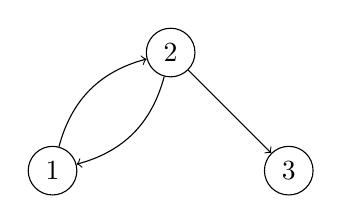
\begin{tikzpicture}[->]
%\begin{tikzpicture}
  \node [draw,circle] (1) at (0,0) {1};
  \node [draw,circle] (2) at (1.5,1.5) {2};
  \node [draw,circle] (3) at (3,0) {3};
  \draw[->,bend left=30] (1) edge (2);
  \draw[->,bend left=30] (2) edge (1);
  \draw (2) -> (3);
\end{tikzpicture}
\caption{Figure F TODO: add caption}
\end{figure}

For edge $(u,v)$, we say that $u$ is the source vertex and $v$ is target vertex; both
$u$ and $v$ are called endpoints.

Subgraph, isomorphism, and maximum common induced subgraph are defined
analogously to the undirected version.

% \section{Generalised Maximum Common Induced Subgraph}
% 
% We now introduce a problem that generalises all three of the problems discussed
% so far. We introduce the concept of a \emph{generalised graph (g-graph)}. A
% g-graph $G = (V, E)$ has a vertex set $V$ and edge set $E$. Each edge in $E$ is
% non-empty tuple of non-empty subsets of $V$. An example of a g-graph with five
% vertices and three edges is
% \[
% (\{1,2,3,4,5\}, \{(\{1,2\},\{4\}), (\{1,2\}), (\{3\},\{4\})\}).
% \]
% 
% If we restrict elements of E to be 1-tuples of 2-element sets, then g-graphs
% are equivalent to graphs. If we remove the upper bound on set size, g-graphs
% become equivalent to hypergraphs. If instead we restrict elements of E to be
% 2-tuples of singleton sets, then g-graphs are equivalent to directed graphs.
% 
% G-graphs can model other types of object such as directed hypergraphs \cite{DBLP:journals/dam/GalloLP93} and a generalisation of directed graphs
% where each edge may be a path of two or more vertices.
% 
% Isomorphism and induced subgraph are defined analogously to their graph
% versions. We call the MCIS problem on g-graphs generalised maximum common
% induced subgraph (G-MCIS).

\section{Maximum Common Edge Subgraph Problems}

We now consider the \emph{maximum common edge subgraph (MCES)} family of problems,
beginning with the simple case of undirected graphs. An edge subgraph of $(V, E)$
is any graph $(W, F)$ such that $W$ is a subset of $V$ and $F$ is a subset of $E$; the
subgraph may thus contain any subsets of the vertices and edges of the original
graph, as long as the subgraph’s vertex set contains all of the endpoints of
edges in its edge set. To give two examples, both graphs in Figure C are edge
subgraphs of the graph in Figure B. Every induced subgraph of a graph $G$ is also
an edge subgraph of $G$.

A common edge subgraph of graphs $G$ and $H$ is an edge subgraph of $G$ that is
isomorphic to an edge subgraph of $H$. A maximum common edge subgraph of two
graphs is a common edge subgraph with as many edges as possible.

?? Chemistry application

%We can extend the definition of MCES to g-graphs to give the G-MCES problem.
%Analogously to its induced counterpart, this has maximum common edge subgraph
%in directed graphs and maximum common edge sub-hypergraph as special cases.

\section{Variants}

Maximum common subgraph problems may be extended by associating a label
function with each graph, which maps each vertex and each edge to a value. The
isomorphism between subgraphs is required to be label-preserving.

?? Loops

\section{Related Problems}

MCIS generalises the induced subgraph isomorphism problem, which is the problem
of determining whether graph $G$ is isomorphic to an induced subgraph of graph $H$.
MCES generalises the non-induced subgraph isomorphism problem, which is to
determine whether $G$ is isomorphic to an edge subgraph of $H$. Both problems are
NP-complete; thus, all of the maximum common subgraph problems described so far
are NP-hard.

Both of the subgraph isomorphism problems generalise graph isomorphism, which
is to determine whether two graphs are isomorphic. ?? As we will discuss later,
our partitioning algorithms have similarities to graph isomorphism algorithms
such as Conauto.

The maximum clique problem is to find an induced subgraph of a graph $G$ with as
many vertices as possible, such that the subgraph has all possible edges; that
is ??. Maximum clique can be solved (although rather inefficiently in practice)
using an MCIS algorithm, by finding the MCIS of $G$ and a complete graph with the
same number of vertices as $G$.

\section{Existing Algorithms}

In this subsection, we outline the existing approaches for solving MCIS on
undirected graphs. Algorithms for other maximum common subgraph problems have
similarities to these approaches, and will be described in detail in later
chapters.

It is useful to introduce the concept of a mapping to denote a pair of common
subgraphs of input graphs $G$ and $H$ and the isomorphism between these subgraphs.
A mapping $M$ is a set of 2-tuples, where each tuple contains a vertex from the
first graph followed by a vertex from the second graph. The subgraph of $G$ is
induced by $\{u \mid (u, v) \in M\}$, and the subgraph of $H$ is induced by $\{v \mid (u, v)
\in M\}$. The isomorphism between these subgraphs is a function that maps each $u$
that appears as the first element of a 2-tuple to the second element of that
tuple.

The association graph of $G$ and $H$ is a graph with $\{(u,v) \mid u \in V(G) \wedge v \in
V(H)\}$ as its vertex set; it thus has $|V(G)||V(H)|$ vertices. Two vertices $(u,v)$
and $(u',v')$ in the association graph are adjacent if and only if all of the
following conditions are met.

\begin{itemize}
  \item $u \not= u'$
  \item $v \not= v'$
  \item $((u,u') \in E(G)) = ((v,v') \in E(H))$
\end{itemize}

A subset of the vertices of the association graph is a valid mapping if and
only if it is a clique in the association graph (?? proof?). Thus, we can find
an MCIS of G and H by running a maximum clique solver on the association graph
of G and H. Association graph encodings can be used to solve directed MCIS on
directed graphs and (with modifications) MCES.

\section{Backtracking Search}

TODO: describe search tree, CP, forward checking, levels of consistency.

\newsavebox{\FourQueensBoxA}
\newsavebox{\FourQueensBoxB}
\newsavebox{\FourQueensBoxC}
\newsavebox{\FourQueensBoxD}
\newsavebox{\FourQueensBoxE}
\newsavebox{\FourQueensBoxF}
\newsavebox{\FourQueensBoxG}
\newsavebox{\FourQueensBoxH}
\newsavebox{\FourQueensBoxI}
\sbox{\FourQueensBoxA}{\FourQueens{A}{0.5/0.5/,1.5/0.5/,2.5/0.5/,3.5/0.5/,0.5/1.5/,1.5/1.5/,2.5/1.5/,3.5/1.5/,0.5/2.5/,1.5/2.5/,2.5/2.5/,3.5/2.5/,0.5/3.5/,1.5/3.5/,2.5/3.5/,3.5/3.5/}}
\sbox{\FourQueensBoxB}{\FourQueens{B}{0.5/0.5/\symqueen,1.5/0.5/$\times$,2.5/0.5/$\times$,3.5/0.5/$\times$,0.5/1.5/$\times$,1.5/1.5/$\times$,2.5/1.5/,3.5/1.5/,0.5/2.5/$\times$,1.5/2.5/,2.5/2.5/$\times$,3.5/2.5/,0.5/3.5/$\times$,1.5/3.5/,2.5/3.5/,3.5/3.5/$\times$}}
\sbox{\FourQueensBoxC}{\FourQueens{C}{0.5/0.5/\symqueen,1.5/0.5/$\times$,2.5/0.5/$\times$,3.5/0.5/$\times$,0.5/1.5/$\times$,1.5/1.5/$\times$,2.5/1.5/\symqueen,3.5/1.5/$\times$,0.5/2.5/$\times$,1.5/2.5/$\times$,2.5/2.5/$\times$,3.5/2.5/$\times$,0.5/3.5/$\times$,1.5/3.5/,2.5/3.5/$\times$,3.5/3.5/$\times$}}
\sbox{\FourQueensBoxD}{\FourQueens{D}{0.5/0.5/\symqueen,1.5/0.5/$\times$,2.5/0.5/$\times$,3.5/0.5/$\times$,0.5/1.5/$\times$,1.5/1.5/$\times$,2.5/1.5/$\times$,3.5/1.5/\symqueen,0.5/2.5/$\times$,1.5/2.5/,2.5/2.5/$\times$,3.5/2.5/$\times$,0.5/3.5/$\times$,1.5/3.5/$\times$,2.5/3.5/,3.5/3.5/$\times$}}
\sbox{\FourQueensBoxE}{\FourQueens{E}{0.5/0.5/\symqueen,1.5/0.5/$\times$,2.5/0.5/$\times$,3.5/0.5/$\times$,0.5/1.5/$\times$,1.5/1.5/$\times$,2.5/1.5/$\times$,3.5/1.5/\symqueen,0.5/2.5/$\times$,1.5/2.5/$\times$,2.5/2.5/\symqueen,3.5/2.5/$\times$,0.5/3.5/$\times$,1.5/3.5/$\times$,2.5/3.5/$\times$,3.5/3.5/$\times$}}
\sbox{\FourQueensBoxF}{\FourQueens{F}{0.5/0.5/$\times$,1.5/0.5/\symqueen,2.5/0.5/$\times$,3.5/0.5/$\times$,0.5/1.5/$\times$,1.5/1.5/$\times$,2.5/1.5/$\times$,3.5/1.5/,0.5/2.5/,1.5/2.5/$\times$,2.5/2.5/,3.5/2.5/$\times$,0.5/3.5/,1.5/3.5/$\times$,2.5/3.5/,3.5/3.5/}}
\sbox{\FourQueensBoxG}{\FourQueens{G}{0.5/0.5/$\times$,1.5/0.5/\symqueen,2.5/0.5/$\times$,3.5/0.5/$\times$,0.5/1.5/$\times$,1.5/1.5/$\times$,2.5/1.5/$\times$,3.5/1.5/\symqueen,0.5/2.5/,1.5/2.5/$\times$,2.5/2.5/$\times$,3.5/2.5/$\times$,0.5/3.5/,1.5/3.5/$\times$,2.5/3.5/,3.5/3.5/$\times$}}
\sbox{\FourQueensBoxH}{\FourQueens{H}{0.5/0.5/$\times$,1.5/0.5/\symqueen,2.5/0.5/$\times$,3.5/0.5/$\times$,0.5/1.5/$\times$,1.5/1.5/$\times$,2.5/1.5/$\times$,3.5/1.5/\symqueen,0.5/2.5/\symqueen,1.5/2.5/$\times$,2.5/2.5/$\times$,3.5/2.5/$\times$,0.5/3.5/$\times$,1.5/3.5/$\times$,2.5/3.5/,3.5/3.5/$\times$}}
\sbox{\FourQueensBoxI}{\FourQueens{I}{0.5/0.5/$\times$,1.5/0.5/\symqueen,2.5/0.5/$\times$,3.5/0.5/$\times$,0.5/1.5/$\times$,1.5/1.5/$\times$,2.5/1.5/$\times$,3.5/1.5/\symqueen,0.5/2.5/\symqueen,1.5/2.5/$\times$,2.5/2.5/$\times$,3.5/2.5/$\times$,0.5/3.5/$\times$,1.5/3.5/$\times$,2.5/3.5/\symqueen,3.5/3.5/$\times$}}

\begin{figure}[h!]
\centering
\begin{forest}
[\usebox{\FourQueensBoxA}
  [\usebox{\FourQueensBoxB}
    [\usebox{\FourQueensBoxC}]
    [\usebox{\FourQueensBoxD} [\usebox{\FourQueensBoxE}]]
  ]
  [\usebox{\FourQueensBoxF}
    [\usebox{\FourQueensBoxG}
      [\usebox{\FourQueensBoxH}
        [\usebox{\FourQueensBoxI}]
      ]
    ]
  ]
]
\end{forest}
\caption{TODO}
\label{fig:FourQueens}
\end{figure}

\newsavebox{\MCSDomainsBoxA}
\newsavebox{\MCSDomainsBoxB}
\newsavebox{\MCSDomainsBoxC}
\newsavebox{\MCSDomainsBoxD}
\sbox{\MCSDomainsBoxA}{\MCSDomains{A}{0.5/4.5/,1.5/4.5/,2.5/4.5/,3.5/4.5/,4.5/4.5/,5.5/4.5/,0.5/3.5/,1.5/3.5/,2.5/3.5/,3.5/3.5/,4.5/3.5/,5.5/3.5/,0.5/2.5/,1.5/2.5/,2.5/2.5/,3.5/2.5/,4.5/2.5/,5.5/2.5/,0.5/1.5/,1.5/1.5/,2.5/1.5/,3.5/1.5/,4.5/1.5/,5.5/1.5/,0.5/0.5/,1.5/0.5/,2.5/0.5/,3.5/0.5/,4.5/0.5/,5.5/0.5/}}
\sbox{\MCSDomainsBoxB}{\MCSDomains{B}{0.5/4.5/M,1.5/4.5/$\times$,2.5/4.5/$\times$,3.5/4.5/$\times$,4.5/4.5/$\times$,5.5/4.5/$\times$,0.5/3.5/$\times$,1.5/3.5/$\times$,2.5/3.5/$\times$,3.5/3.5/,4.5/3.5/$\times$,5.5/3.5/,0.5/2.5/$\times$,1.5/2.5/$\times$,2.5/2.5/$\times$,3.5/2.5/,4.5/2.5/$\times$,5.5/2.5/,0.5/1.5/$\times$,1.5/1.5/,2.5/1.5/,3.5/1.5/$\times$,4.5/1.5/,5.5/1.5/$\times$,0.5/0.5/$\times$,1.5/0.5/,2.5/0.5/,3.5/0.5/$\times$,4.5/0.5/,5.5/0.5/$\times$}}
\sbox{\MCSDomainsBoxC}{\MCSDomains{C}{0.5/4.5/M,1.5/4.5/$\times$,2.5/4.5/$\times$,3.5/4.5/$\times$,4.5/4.5/$\times$,5.5/4.5/$\times$,0.5/3.5/$\times$,1.5/3.5/$\times$,2.5/3.5/$\times$,3.5/3.5/M,4.5/3.5/$\times$,5.5/3.5/$\times$,0.5/2.5/$\times$,1.5/2.5/$\times$,2.5/2.5/$\times$,3.5/2.5/$\times$,4.5/2.5/$\times$,5.5/2.5/,0.5/1.5/$\times$,1.5/1.5/$\times$,2.5/1.5/$\times$,3.5/1.5/$\times$,4.5/1.5/,5.5/1.5/$\times$,0.5/0.5/$\times$,1.5/0.5/,2.5/0.5/,3.5/0.5/$\times$,4.5/0.5/$\times$,5.5/0.5/$\times$}}
\sbox{\MCSDomainsBoxD}{\MCSDomains{D}{0.5/4.5/M,1.5/4.5/$\times$,2.5/4.5/$\times$,3.5/4.5/$\times$,4.5/4.5/$\times$,5.5/4.5/$\times$,0.5/3.5/$\times$,1.5/3.5/$\times$,2.5/3.5/$\times$,3.5/3.5/M,4.5/3.5/$\times$,5.5/3.5/$\times$,0.5/2.5/$\times$,1.5/2.5/$\times$,2.5/2.5/$\times$,3.5/2.5/$\times$,4.5/2.5/$\times$,5.5/2.5/M,0.5/1.5/$\times$,1.5/1.5/$\times$,2.5/1.5/$\times$,3.5/1.5/$\times$,4.5/1.5/$\times$,5.5/1.5/$\times$,0.5/0.5/$\times$,1.5/0.5/,2.5/0.5/,3.5/0.5/$\times$,4.5/0.5/$\times$,5.5/0.5/$\times$}}

\begin{figure}[h!]
\centering
\begin{forest}
[\usebox{\MCSDomainsBoxA}
  [\usebox{\MCSDomainsBoxB}
    [\usebox{\MCSDomainsBoxC}
      [\usebox{\MCSDomainsBoxD}]%[$\dots$]
    ]
    %[$\dots$]
  ]
  %[$\dots$]
]
\end{forest}
\caption{TODO}
\label{fig:MCSDomains}
\end{figure}

\section{Branch and Bound}

All of the maximum common subgraph problems discussed in this paper are
optimisation problems.  Branch and bound is a general technique for solving
optimisation problems by backtracking search. We will describe branch and bound
in the context of maximisation (rather than minimisation) problems.

During search, we maintain an incumbent---the best solution found so far. Each
time a solution $S$ whose objective value is larger than the incumbent is found,
the incumbent’s value is updated to $S$. At each search node we calculate an
upper bound on the best objective value that can be obtained by extending the
current partial solution. If this upper bound is not greater than the
incumbent’s objective value, we know that exploring the subtree below the
current search node would be fruitless, and we therefore backtrack.

An alternative to branch and bound is to solve the maximisation problem by a
sequence of decision problems. Beginning at a known upper bound $B$ for the
optimal objective value, we use search to answer the question “does a solution
with objective value B exist?” If the answer is “yes”, the algorithm
terminates. Otherwise, a solution with objective value $B-1$ is sought, then $B-2$,
and so on until a solution is found.

A third alternative for solving optimisation problems, which again involves a
sequence of decision problems, is binary search on the objective value. Begin
with a known lower bound $L$ and a known upper bound $B$ for the objective value.
(For MCIS, we could trivally use $L=0$ and $B=|V(G)|$.) ?? Then do binary search to
find the largest objective value for which the decision problem is satisfiable.
Cite the book cited in the Handbook of CP. Say why we don’t try this approach
in this thesis.  Say what this approach would gain us.

\section{Inexact Algorithms}

TODO

\section{Algorithms for Subgraph Isomorphism} 

TODO introduce this section. Also mention graph databases and indexing?

\citet{sussenguth1965graph} presents one of the earliest algorithms for
induced subgraph isomorphism.  The algorithm uses a variety of vertex properties
to generate pairs of sets of vertices $\langle S_G, S_H \rangle$
such that $S_G \subseteq V(G)$, $S_H \subseteq V(H)$,
and each vertex in $S_G$ may only be mapped to some member of $S_H$.
For example, the vertices in in the pattern graph of degree 3 may only be mapped to vertices
in the target graph of degree at least 3.  Other properties used include
vertex labels and the size of the smallest cycle containing a vertex.
Further reasoning is performed based on adjacency to members of these
sets $S_G$ and $S_H$.  Certainly Sussenguth's algorithm has a strong
constraint-programming flavour, albeit without storing each domain
individually.  (To preview the family of algorithms presented
in this dissertation, the \McSplit\ algorithm shares with Sussenguth's
algorithm the approach of storing
pairs of sets $\langle S_G, S_H \rangle$ respresenting vertices
that may be mapped to one another. However, \McSplit\ uses a very different
data structure to store these sets, taking advantage of the fact the
sets used by \McSplit\ are guaranteed to be disjoint.)

\subsection{Algorithms based on constraint programming}

\paragraph*{Ullmann} 
The algorithm of \citet{ullmann1976algorithm} 
is the first subgraph isomorphism algorithm based on constraint programming.
The paper only considers the non-induced version of subgraph isomorphism,
but the algorithm could easily be extended to the induced variant by adding
constraints to ensure non-adjacent vertices are mapped to non-adjacent vertices.
The algorithm maintains arc consistency on the adjacency constraints.

\paragraph*{McGregor}
\citet{DBLP:journals/isci/McGregor79} introduces a modified version of
Ullmann's algorithm.  McGregor finds experimentally that the cost of maintaining
arc consistency throughout search outweighs the benefit; as a compromise,
McGregor enforces arc consistency only after assigning the first pattern-graph
vertex, and uses forward checking at deeper levels of the search tree.
McGregor uses a static variable ordering heuristic in which vertices
with most constraints to previously-instantiated vertices are selected first.

\paragraph*{R{\'{e}}gin's all-different propagator}
\citet{DBLP:conf/aaai/Regin94}
introduced a filtering algorithm for the all-different constraint that
ensures generalised arc consistency.  The algorithm removes from each domain
$D$ each value $x$ such that there exists no assignment of distinct
values to all of the variables in which $D$ takes the value $x$.
R{\'{e}}gin reports that this filtering algorithm was used to solve
the subgraph isomorphism problem in the RESYN system \citep{vism92}.
TODO maybe mention his thesis (cited in LAD paper)

\paragraph*{ILF(k)} \citep(DBLP:journals/constraints/ZampelliDS10)
introduces a filtering algorithm based on assigning during
search a label
to each vertex of the pattern graph and the target graph, with a partial ordering
$\preccurlyeq$ over the labels such that $v \in \V(G)$ may be assigned to $w \in V(H)$
if and only if $\mathit{label}(v) \preccurlyeq \mathit{label}(w)$.
Labels are iteratively extended to include information about the labels of
neighbouring vertices.
Although this algorithm is described and implemented
only for the non-induced version of
subgraph isomorphism, it appears that it could be extended to solve
the induced variant.  Like ILF(k), the McSplit family of algorithms
described in this dissertation may be viewed as assigning a label
to each vertex and requiring that only vertices with compatible labels
be assigned to one another. Unlike ILF(k), however, McSplit requires
labels to equal.  While this severly restricts the information that the
McSplit labels may contain, it results in very fast and simple constraint
propagation in the McSplit algorithm.

\paragraph*{LAD}
\citet{DBLP:journals/ai/Solnon10} proposes an algorithm for
LAD (local all different) filtering,
which propagates the following constraint:
if $v \in V(G)$ is mapped to $w \in V(H)$, then the neighbours of $v$ in $G$
must all be mapped to different values, and these values must all belong to
the set $N_H(w)$.
This strengtens the filtering of the nRF+ algorithm \citep{DBLP:journals/mscs/LarrosaV02},
and can be performed in $O(|V(G)| \cdot |V(H)| \cdot \Delta_G^2 \cdot \Delta_H^2)$
time, where $\Delta_G$ and $\Delta_H$
are the maximum degrees of $G$ and $H$.

\paragraph*{SND}
The SND algorithm \citep{DBLP:conf/cp/AudemardLMGP14}
extends LAD by counting the number of length-$k$ paths between
pairs of vertices for small values of $k$, and enforcing within
a LAD-style constraint that 
a pair of pattern vertices connected by $p$ paths of lenght $k$
may not be mapped to a pair of target vertices connected by fewer
than $p$ paths of length $k$.
PathLAD \citep{DBLP:conf/lion/KotthoffMS16} incorporates a subset
of the SND filtering into the LAD algorithm.

\paragraph*{Symmetry breaking}
\citet{zampelli2007symmetry} show that the variable and value symmetries
in the subgraph isomorphism problem can be completely broken using
the automorphism groups of the pattern and target graph graphs.
Moreover, the authors show how to break local symmetries that emerge
during search.
This work was extended in Zampelli's PhD thesis \citep{DBLP:phd/basesearch/Zampelli08}.
A solver with symmetry breaking was shown to be able to solve many more instances
than the same solver without symmetry breaking. 
Techniques based on those of \citeauthor{zampelli2007symmetry} 
could be applied to any subgraph isomorphism solver based on constraint programming,
and the use of such techniques is understudied; neither McSplit-SI nor any of
the state-of-the-art algorithms to which we compare it in our experiments
uses symmetry breaking.  This appears to be a fruitful area for future
work.

\paragraph*{SubGlw}
Finally, for completeness, we describe the SubGlw solver \citep{DBLP:journals/access/AnsariJA21},
which solves an incomplete enumeration problem: the problem of
generating up to $k$ subgraph embeddings within a given time limit, for a given
parameter $k$. To do this efficiently, the solver chooses a promising
subgraph $S$ of the target graph, and runs the Glasgow Subgraph Solver in enumeration
mode with pattern graph $G$ and target graph $S$. This avoids the overhead of
building up the Glasgow solver's supplemental graph data structures for a large
graph.  Since SubGlw is a small wrapper around an existing solver, and because
it solves an incomplete enumeration problem that is not considered further
in this thesis, we do not include it in our experimental evaluation.

\subsection{Pattern recognition algorithms}

Algorithms for subgraph isomorphism from the pattern recognition (PR) community
take a different approach from solvers based on constraint programming.  PR
solvers take a lightweight approach --- they do not store domains and perform
minimal work at each search node, resulting in algorithms with very low memory
requirements that can visit many search nodes per second, but often have to
visit many more search nodes in total than CP algorithms.

TODO write more. Maybe cut and paste from McSplit-SI chapter?

\subsection{Other approaches}

\citet{DBLP:conf/RelMiCS/CortadellaV00} represent an instance of the subgraph
isomorphism problem as a binary decision diagram (BDD), and solve this BDD
in order to find all solutions to the subgraph isomorphism problem.  A limitation
is that for large
pattern graphs, the size of the BDDs quickly becomes unmanageable; the experiments
in the paper only consider pattern graphs with 10 or fewer vertices.

\section{Algorithms for Maximum Common Subgraph} 

\textbf{TODO see \citet{DBLP:journals/jcamd/RaymondW02a} for a helpful lit review.
Also Duesbury Holliday and Willett review}

Exact algorithms for the maximum common induced subgraph problem may be divided
into three broad categories:
algorithms that solve the maximum clique problem for the association graph,
algorithms based on constraint programming,
and algorithms that enumerate subgraphs of graph $G$ and use a subgraph
isomorphism algorithm to search for each subgraph in graph $H$.  We now review
each of these categories.

\subsection{Clique algorithms}

\citet{LeviG} reformulated the maximum common induced subgraph problem as the problem
of finding a maximum clique in the association graph of $G$ and $H$.

The RASCAL algorithm \citep{raymond2002rascal} solves MCES by finding a maximum
clique in the modular product graph of the line graphs.  The algorithm is
optimised for matching chemical structures, and does not solve the maximum common
\emph{connected} subgraph problem.  In addition to greedy
colouring, the algorithm uses a number of other heuristic colourings to derive
an upper bound depending on the size of the modular product graph.  Unfortunately
the authors were unable to provide code for RASCAL.

\cite{DBLP:conf/cp/McCreeshNPS16} uses a state of the art maximum clique algorithm
to solve this problem, and introduces a modified version of the algorithm to
solve maximum common \emph{connected} induced subgraph.

\subsection{Constraint programming algorithms}

\citet{DBLP:journals/spe/McGregor82}
introduced a branch and bound algorithm for the maximum common
\emph{edge} subgraph problem in which a vertex of $G$ is mapped to a vertex
of $H$ at each node of the search tree.  A matrix of boolean values indicates
the set of edges in $H$ to which each edge in $G$ may be mapped; this may be
viewed as a simple domain store. \citet{DBLP:conf/sspr/BunkeFGSV02}
reports using McGregor's algorithm to solve MCIS, without giving full
details of the modifications made to the algorithm.

The first formal CP model for MCIS is given by \cite{DBLP:conf/mco/VismaraV08}.
This uses binary constraints between all pairs of variables to ensure that
no pair of vertices in $G$ are mapped to the same vertex in $H$.

\citet{DBLP:conf/cp/NdiayeS11} present a CP model that shares the variables
of the \citeauthor{DBLP:conf/mco/VismaraV08} model, but replaces the binary constraints
described above with a single global ``soft allDiff''
constraint \citep{DBLP:conf/cp/PetitRB01}.  This ensures that distinct vertices
in $G$ are mapped to distinct vertices in $H$, and uses a matching algorithm
to calculate a stronger upper bound than the one given by
the \citeauthor{DBLP:conf/mco/VismaraV08} model.
\citeauthor{DBLP:conf/cp/NdiayeS11} carry out detailed experiments using
different levels of consistency for the adjacency and soft allDiff constraints.
The soft allDiff constraint, which used to calculate an upper bound but
not to filter domains, causes the algorithm to run several times faster
than the simple difference constraints used by \citeauthor{DBLP:conf/mco/VismaraV08}.
Comparing forward checking (FC) and maintaining arc consistency (MAC)
on the adjacency constraints, FC outperforms MAC on unlabelled instances
while MAC outperforms FC on labelled instances.

\cite{DBLP:conf/cp/McCreeshNPS16} add a connectedness constraint to
the CP model of \citet{DBLP:conf/cp/NdiayeS11}.  This is found to perform
better overall than simply branching on vertices adjacent to some already-mapped
vertex in order to ensure connectedness.

\subsection{Subgraph enumeration algorithms}

Finally, we mention briefly a very different technique that has been used
in a number of papers to find a maximum common connected subgraph between two or more
graphs representing molecules.
\citep{armitage1967automatic}
\citep{takahashi1987recognition}
\citep{DBLP:journals/jcheminf/DalkeH13}
In this type of algorithm, connected
subgraphs of the first graph are built one node at a time by a tree search.
A subgraph isomorphism solver is used to test whether each of these subgraphs
appears in each of the other input graphs.  In some versions of this algorithms,
the subgraphs of $G$ are tested for isomorphism with previously-generated subgraphs
in order to break symmetries.
Unfortunately, we have been unable to find an implementation of this technique
for MCIS in general graphs to use in our experimental evaluation.

\subsection{Misc stuff to sort out}

\citet{cao2008maximum} is a backtracking algorithm that does not store domains,
but tests before making each assignment $(v,w)$ whether the set of vertices in $M$
that are adjacent to $v$ in $G$ corresponds to the set of vertices in $M$ that
are adjacent to $w$ in $H$.  The main upper bound proposed by the authors
is, in CP terms, the bound given by adding to $|M|$ the number of unassigned
variables whose domains contain at least one vertex.  The authors also outline
a matching upper bound.  In each case, it appears likely that the fact that the algorithm does not
store domains results in substantial addition work on each call of the upper bound
function.  (TODO tidy up that last sentence!)

\citet{DBLP:conf/cp/McCreeshNPS16} TODO talk about clique algo, new version
of clique algo for connected. TODO check: do they introduce a new connected
constraint? Do I compare against this in McSplit chapter?

\section{New algorithms in this thesis}

The McSplit family of algorithms has branch-and-bound variants and variants
that use a sequence of decision problems; it also has variants for induced and
edge subgraph problems. The summary in this section discusses only the induced
variants.

McSplit performs tree search in the style of a forward-checking constraint
programming algorithm. Rather than maintaining an explicit domain for each
vertex in the first graph, vertices are re-labelled at each search node in such
a way that the current mapping may only be extended by mapping a vertex in
first graph to a vertex in the second graph with the same label. Labels may be
viewed as equivalence classes of vertices, and at each search node these
classes are refined (partitioned) into smaller classes. We store the vertices
of each graph as a list (without copying at each search node), and can perform
this partitioning efficiently be re-arranging the vertices in each list. This
data structure makes it possible to calculate an upper bound very cheaply at
each search node, and permits the cheap computation of good variable-ordering
heuristics.

\section{Experimental setup}

The experiment in chapters ... were run on ...

The experiments in chapter ... were run on ...

All solvers were compiled using GCC version 9.4.0 with the flags
\texttt{-O3} (optimization level 3) and \texttt{-march=native}
(which allows the compiler to use any CPU instruction that is available
on the machine, and is particularly helpful in improving the performance
of the Glasgow Subgraph Solver).

\section{A Note on Run Time Plots}

TODO Mention jittering, explain cumulative plots. Or do it when first
one is shown?

\section{Structure of the Dissertation}

FIXME

Chapter 2 surveys the literature on algorithms for MCIS, MCES, and related
problems. Chapter 3 introduces the McSplit algorithm for MCIS on undirected
graphs. Chapter 4 generalises McSplit to MCIS problems on g-graphs. In Chapter
5, we turn to MCES, and describe how this can be solved by a variant of McSplit
and by association graph encodings. In Chapter 6, we introduce a variant of
McSplit for block and bridge preserving MCIS, a version of the problem with
applications to chemistry. Chapter 7 concludes.

\section{Miscellaneous notes}

MCIS is NP-hard, even if graphs are both bipartite.  This can be shown by a
reduction from maximum induced matching.  (I think the proof for maximum induced
matchings is in Induced Matchings (1989) by Kathie Cameron). Is there another
proof somewhere?

Independent set is NP-hard on planar graphs (see Wikipedia).  Therefore
MCIS also is.

Cuissart and Hebrard 2005 A Direct Algorithm to Find a Largest Common
Connected Induced Subgraph of Two Graphs doesn't seem to do any
pruning.  Is it slow?

\section{Publications}

During the course of my PhD I carried out further work
that is not presented in this thesis.
For completeness, the following is a full list of publications
since the start of my PhD.  The first of these
forms the basis of \Cref{c:mcsplit-i-undirected}.

\begin{itemize}
    \item\bibentry{DBLP:conf/ijcai/McCreeshPT17}
    \item\bibentry{DBLP:conf/cp/McCreeshPST17}
    \item\bibentry{DBLP:conf/cpaior/HoffmannMNPRS018}
    \item\bibentry{DBLP:journals/jair/McCreeshPST18}
    \item\bibentry{DBLP:conf/cpaior/ArchibaldDHMP019}
    \item\bibentry{DBLP:conf/wea/000120a}
    \item\bibentry{DBLP:conf/iwpec/000120}
    \item\bibentry{DBLP:conf/iwpec/000120a}
    \item\bibentry{DBLP:conf/gg/McCreeshP020}
    \item\bibentry{DBLP:conf/cp/GochtMMNPT20}
    \item\bibentry{DBLP:journals/cor/DelormeGGKMPT22}
\end{itemize}

%==============================================================================
\section{Thesis Statement}
\label{c:intro:thesisstatement}

This dissertation has the following thesis.

\emph{The structure of the induced subgraph isomorphism and maximum common
subgraph problems allows us to use specialised, compressed data structures to
efficiently represent domains in a backtracking algorithm; by using these
structures we can design algorithms that run faster than the existing state of
the art on many instance classes.}

